\documentclass[utf-8]{beamer}
\usepackage{graphicx}
\usepackage{ragged2e}
\usepackage{amsmath}
\usepackage[table]{xcolor}


\graphicspath{{./Resources/images/}}

%title page
\title{Gaussian Blur}
\author[Słupik, Dyrda]{Xawier Słupik \and Adam Dyrda}
\institute{Informatics}
\date{Winter semerster 2026/2027}

\begin{document}

\frame{\titlepage}


\begin{frame}
    \frametitle{What is Gaussian Blur}
    \begin{columns}
    \column{0.5\textwidth}    
        Widely used effect in graphics software
        used to reduce the noise or definition of the image.
        \column{0.5\textwidth}
        
        \begin{figure}
            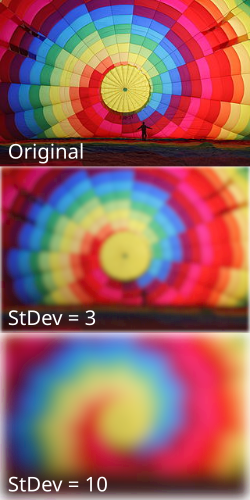
\includegraphics[width=0.6\linewidth]{Gaussian-blur-example.png}
            \caption{example of gaussian blur}
        \end{figure}
    \end{columns}
\end{frame}
\begin{frame}
\frametitle{How it works}
\framesubtitle{Convolution}
\end{frame}


\begin{frame}
\frametitle{How it works}
\framesubtitle{Convolution}
\begin{columns}
    %left column with text
    \column{0.5\textwidth}
    \justifying
    When it comes to blurring the image we use a so-called convolution layer.\\ \vspace{20px}
    In simple words it takes a fragment of the image and blurrs center pixel based on the surrounding ones.
    %right column with pictures
    \column{0.5\textwidth}
    \begin{figure}
        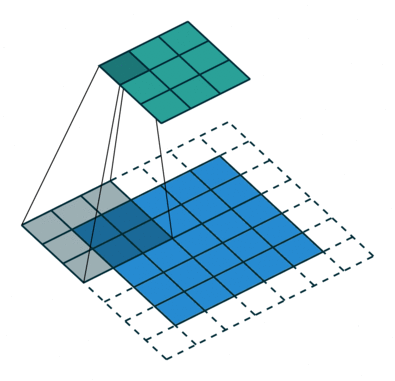
\includegraphics[width=0.35\textwidth]{padding_strides-0.png}
    \end{figure}
    \begin{figure}
        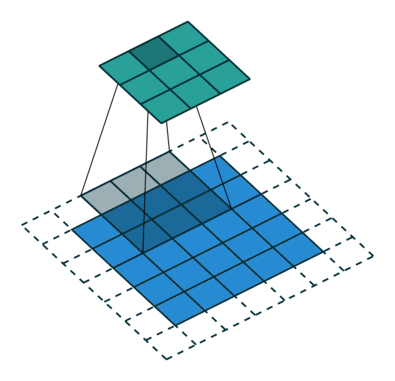
\includegraphics[width=0.35\textwidth]{padding_strides-1.png}
    \end{figure}
    \begin{figure}
        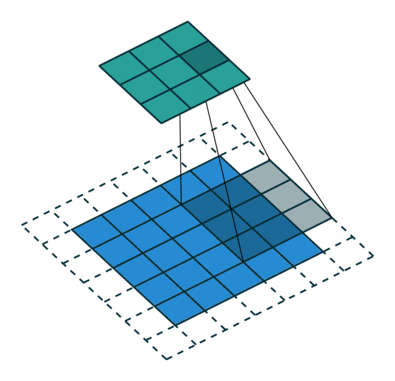
\includegraphics[width=0.35\textwidth]{padding_strides-5.png}
    \end{figure}
\end{columns}
\end{frame}

\begin{frame}
\frametitle{How it works}
\framesubtitle{Kernel Generation}
\begin{columns}
    %left column with text
    \column{0.5\textwidth}
    \justifying
    The convolution layer uses a kernel which is a matrix of the same size as the layer.\\ \vspace{20px}
    The matrix stores pixel weights that are the prime factor when it comes to the final pixel blur.
    %right column with pictures
    \column{0.5\textwidth}
    \begin{figure}
        \centering
        $G(x,y) = \frac{1}{2\pi\sigma^2} e^{-\frac{x^2 + y^2}{2\sigma^2}}$
        \caption{Formula for calculating Gaussian kernel.}
    \end{figure}
    \vspace{-20 px}
    \begin{figure}
    $$
    \begin{bmatrix}
    1 & 2 & 1 \\
    2 & 4 & 2 \\
    1 & 2 & 1
    \end{bmatrix}
    $$
    \caption{Kernel generated by the formula above. Requires normalization.}
    \end{figure}
    
\end{columns}
\end{frame}

\begin{frame}
\frametitle{How it works}
\framesubtitle{Kernel Normalization}
To prevent the image from getting brighter or darker we normalize the kernel,
so all the weights add up to exactly 1.
$$
K= \frac{1}{16} \begin{bmatrix}
    1 & 2 & 1 \\
    2 & 4 & 2 \\
    1 & 2 & 1
    \end{bmatrix}
    =
    \begin{bmatrix}
    0.0625 & 0.125 & 0.0625 \\
    0.125  & 0.25  & 0.125  \\
    0.0625 & 0.125 & 0.0625
    \end{bmatrix}
$$
\end{frame}

\begin{frame}
    \frametitle{Implementation}
    \framesubtitle{Generating 1D kernel}
    The formula for one dimensional gaussian function is:
    \[G(x) = \frac{1}{\sqrt{2\pi\sigma^2}}e^{-\frac{x^2}{2\sigma^2}}\]
    Because the kernel gets normalized by dividing each element by the sum of all elements, the part $\frac{1}{\sqrt{2\pi\sigma^2}}$ can be ommited from the equation, because it cancels out. The leftover equation is: 
    \[G(x) = e^{-\frac{x^2}{2\sigma^2}}\]

\end{frame}
\begin{frame}
    \frametitle{Implementation}
    \framesubtitle{Two-pass seperate convolution}
    \begin{enumerate}
        \item \textbf{Horizontal pass} - for every pixel the 1D kernel slides left-to-right across row y and save the sums to the temp buffer.
        \item \textbf{Vertical pass} - using temp buffer as the new source, the exact same 1D kernel slides top-to-bottom down column x. After this pass is done the output image is obtained.
    \end{enumerate}

\end{frame}

\begin{frame}
    \frametitle{Implementation}
    \framesubtitle{Image loading}
    When it comes to image, each pixel channel [B, G, R, A] is loaded as a 32-bit float giving 4 32-bit values.
    This comes to be ideal for working with SIMD instructions (summing, multiplication, etc.) because the XMM register stores 128 bits and thats exactly 4 float values.
    \begin{table}[h!]
        \centering
        \begin{tabular}{|c|c|c|c|}
            \hline
            \cellcolor{blue!25} BLUE (32) & 
            \cellcolor{green!25} GREEN (32) & 
            \cellcolor{red!25} RED (32) & 
            \cellcolor{yellow!35} ALPHA (32) \\
            \hline
        \end{tabular}
        \caption{128-bit XMM register}
    \end{table}
\end{frame}

\begin{frame}
    \frametitle{Implementation}
    \framesubtitle{Assembler advantages}
    \begin{itemize}
        \item SIMD vectorization
        \item For small kernels, the weights can be preloaded into the dedicated registers.
        \item It's possible to split each scan line into zones, so border clamping can be avoided.
        \item is cooler ;)
    \end{itemize}
\end{frame}

\end{document}